\chapter{Pendekatan Akar Persamaan Satu Variabel}

\section*{Pengantar}
Pada Bab~1 dan Bab~2, kita telah mempelajari persamaan garis lurus serta sifat-sifat fungsi secara umum. Dalam masalah teknik, banyak dijumpai suatu persamaan transenden (sukar dipahami) yang sulit atau belum ditemukan penyelesaian eksaknya. Dengan metode numerik, akar-akar real persamaan $f(x) = 0$ dapat ditentukan secara pendekatan. Berikut ini akan dibahas beberapa metode yang berkenaan dengan pencarian akar persamaan secara pendekatan, termasuk metode grafik dan tabulasi yang memanfaatkan sifat kontinu fungsi, serta metode iteratif penarikan akar.


\section{Metode Grafik dan Tabulasi}
Mula-mula akar persamaan yang akan kita cari kita "tebak". Bila persamaannya mengandung satu variabel, maka akar yang kita tebak tersebut sebaiknya ditentukan dari grafik. Akar ini dikenal sebagai harga awal. Selanjutnya harga awal ini "peralus" dengan metode tabulasi.

Sebagai gambaran, kita akan menyelesaikan persamaan berikut

\begin{equation}
x^4 - 3x - 2 = 0
\end{equation}

Ada dua cara pembuatan grafik untuk menentukan harga awal. Pertama, kita buat satu grafik secara keseluruhan, yakni $y = x^4 - 3x - 2$. Maka harga awal yang kita cari adalah titik potong grafik dengan sumbu $x$. Ternyata seperti yang ditunjukkan pada gambar 1-1(a), ada dua titik potong grafik dengan sumbu $x$. Ini terbukti bahwa persamaan tersebut memiliki 2 akar real.

\begin{figure}[!h]
\centering
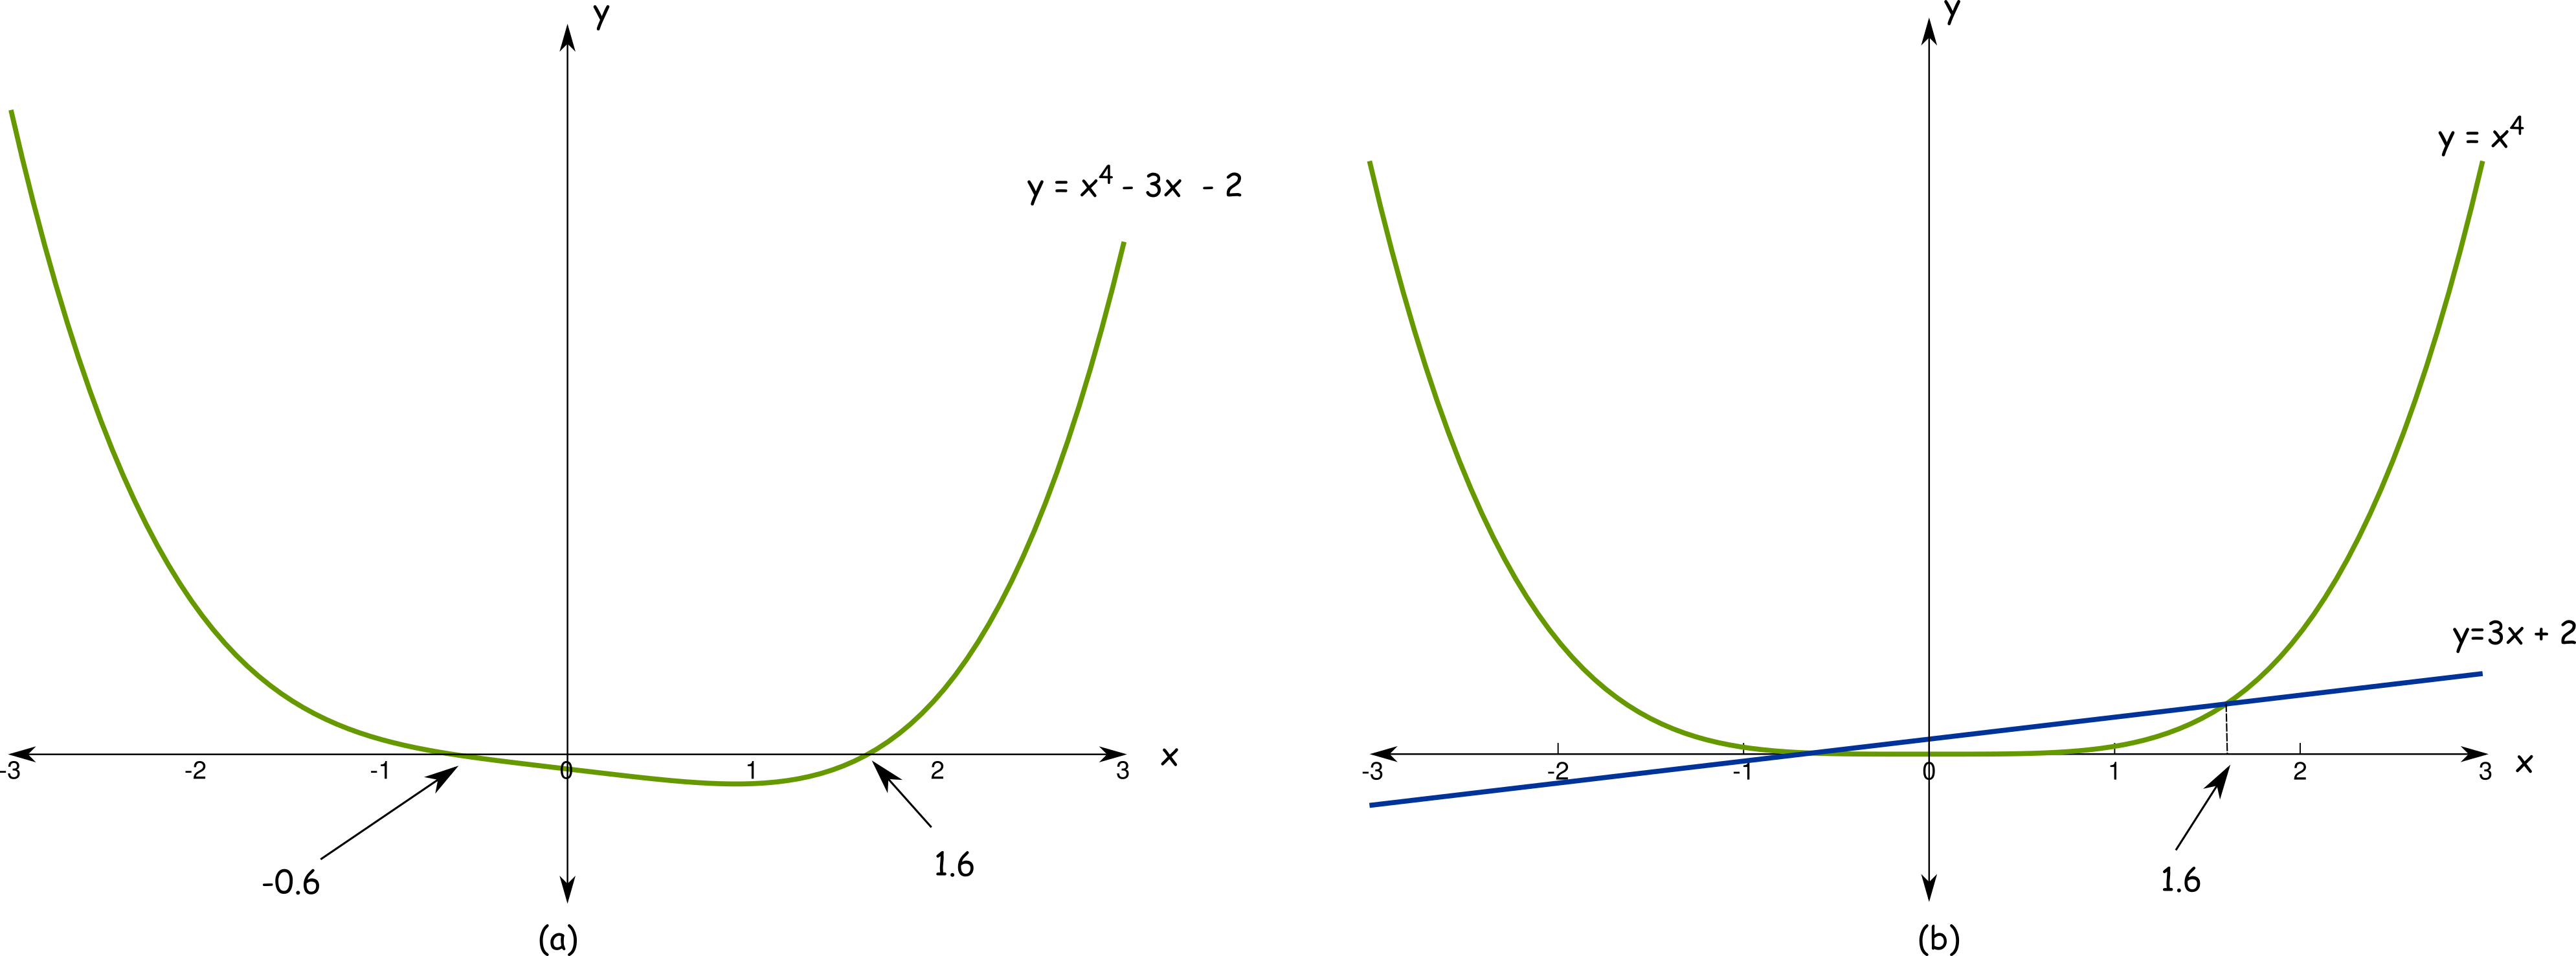
\includegraphics[width=5in]{pict/fig1_1}
\caption{Penentuan harga awal $y=x^4-3x-2$ (a)}\label{gambar1_1}
\end{figure}

Cara kedua adalah persamaan itu kita bagi menjadi dua bagian. Pembagian itu terserah kita, misalnya $y = x^4$ dan $y = 3x + 2$, mula-mula, kita pilah persamaan itu menjadi $x^4 = 3x+2$. Harga awalnya diperoleh dari absis titik potong kedua grafik tersebut. Dari grafik, baik pada gambar 1-1(a), maupun pada gambar 1-1(b) didapat harga awal $-0{,}6$ dan $1{,}6$.


Pada metode tabulasi, kita harus mencari dua buah harga $x$ sedemikian hingga nilai $y = f(x)$ berlainan tanda. Akar sejati berada di antara dua nilai tersebut. Untuk akar yang berlokasi di sekitar harga awal $x \approx -0{,}6$, kita buat tabel berikut dengan langkah $\Delta x = 0{,}01$.

\begin{table}[!htbp]
\centering
\caption{Tabulasi $f(x) = x^4 - 3x - 2$ di sekitar $x = -0{,}6$}
\label{tabel:tabulasi1}
\begin{tabular}{|c|r|}
\hline
$x$ & $f(x) = x^4 - 3x - 2$ \\ \hline
$-0{,}70$ & $\phantom{-}0{,}3401$ \\
$-0{,}69$ & $\phantom{-}0{,}3009$ \\
$-0{,}68$ & $\phantom{-}0{,}2629$ \\
$-0{,}67$ & $\phantom{-}0{,}2261$ \\
$-0{,}66$ & $\phantom{-}0{,}1906$ \\
$-0{,}65$ & $\phantom{-}0{,}1565$ \\
$-0{,}64$ & $\phantom{-}0{,}0878$ \\
$-0{,}63$ & $\phantom{-}0{,}0475$ \\
$-0{,}62$ & $\phantom{-}0{,}0078$ \\
$-0{,}61$ & $-0{,}0315$ \\ \hline
\end{tabular}
\end{table}

Dari Tabel~\ref{tabel:tabulasi1} terlihat bahwa $f(x)$ berganti tanda antara $x = -0{,}62$ (positif) dan $x = -0{,}61$ (negatif). Artinya akar berada dalam interval $[-0{,}62,\, -0{,}61]$. Dengan mengulang proses tabulasi menggunakan langkah yang lebih kecil ($\Delta x = 0{,}001$) pada interval tersebut, kita akan mendapatkan pendekatan akar yang lebih akurat, misalnya $x \approx -0{,}618$.

Dengan cara yang sama, akar kedua yang berada di sekitar harga awal $x \approx 1{,}6$ dapat dicari dengan membuat tabel tabulasi di sekitar nilai tersebut. Hasil yang diperoleh adalah $x \approx 1{,}602$.


\section{Sistem Penarikan Akar}

Selain metode grafik dan tabulasi, pencarian akar juga dapat dilakukan melalui \textbf{sistem penarikan akar} secara iteratif. Metode ini sangat berguna untuk menghitung akar kuadrat, akar pangkat tiga, atau akar pangkat-$n$ dari suatu bilangan secara numerik.

\subsection{Metode Heron (Metode Babilonia)}

Metode Heron adalah metode iteratif tertua untuk menghitung akar kuadrat $\sqrt{a}$, yaitu mencari $x$ sehingga $x^2 = a$. Rumus iterasinya adalah:
\begin{equation}
x_{n+1} = \frac{1}{2}\left(x_n + \frac{a}{x_n}\right),
\end{equation}
dengan $x_0 > 0$ sebagai tebakan awal.

\textbf{Prinsip kerja:} Jika $x_n$ terlalu besar sebagai pendekatan $\sqrt{a}$, maka $a/x_n$ terlalu kecil, dan sebaliknya. Rata-rata keduanya memberikan pendekatan yang lebih baik.

\begin{exmp}
Hitunglah $\sqrt{2}$ menggunakan metode Heron dengan $x_0 = 1$!

\textbf{Penyelesaian:}\\
\begin{align*}
x_0 &= 1{,}000000 \\
x_1 &= \frac{1}{2}\left(1 + \frac{2}{1}\right) = 1{,}500000 \\
x_2 &= \frac{1}{2}\left(1{,}5 + \frac{2}{1{,}5}\right) = 1{,}416667 \\
x_3 &= \frac{1}{2}\left(1{,}416667 + \frac{2}{1{,}416667}\right) = 1{,}414216 \\
x_4 &= 1{,}414214
\end{align*}
Hanya dalam empat iterasi, kita sudah mendapatkan $\sqrt{2} \approx 1{,}414214$ yang akurat hingga enam desimal.
\end{exmp}

\subsection{Metode Newton--Raphson untuk Penarikan Akar}

Metode Heron sesungguhnya merupakan kasus khusus dari \textbf{metode Newton--Raphson}. Untuk mencari akar kuadrat $\sqrt{a}$, kita definisikan fungsi $f(x) = x^2 - a$ sehingga akar fungsi ini adalah $x = \sqrt{a}$. Metode Newton--Raphson memberikan rumus iterasi umum:
\begin{equation}
x_{n+1} = x_n - \frac{f(x_n)}{f'(x_n)}.
\end{equation}

Untuk $f(x) = x^2 - a$, kita peroleh $f'(x) = 2x$, sehingga:
\[
x_{n+1} = x_n - \frac{x_n^2 - a}{2x_n} = \frac{1}{2}\left(x_n + \frac{a}{x_n}\right),
\]
yang identik dengan rumus Heron.

\subsection{Penarikan Akar Pangkat-$n$}

Untuk menghitung $\sqrt[n]{a}$, kita definisikan $f(x) = x^n - a$, sehingga $f'(x) = nx^{n-1}$. Rumus iterasi Newton--Raphson menjadi:
\begin{equation}
x_{k+1} = \frac{1}{n}\left[(n-1)\,x_k + \frac{a}{x_k^{n-1}}\right].
\end{equation}

\begin{exmp}
Hitunglah $\sqrt[3]{10}$ menggunakan rumus iterasi di atas dengan $x_0 = 2$!

\textbf{Penyelesaian:}\\
Dengan $n = 3$ dan $a = 10$:
\[
x_{k+1} = \frac{1}{3}\left(2x_k + \frac{10}{x_k^2}\right).
\]
\begin{align*}
x_0 &= 2{,}000000 \\
x_1 &= \frac{1}{3}\left(4 + \frac{10}{4}\right) = \frac{1}{3}(6{,}5) = 2{,}166667 \\
x_2 &= \frac{1}{3}\left(4{,}333334 + \frac{10}{4{,}694445}\right) = 2{,}154504 \\
x_3 &= 2{,}154435
\end{align*}
Nilai eksak: $\sqrt[3]{10} = 2{,}154435\ldots$ Konvergensi tercapai dalam tiga iterasi.
\end{exmp}

\subsection{Laju Konvergensi}

Metode Newton--Raphson untuk penarikan akar memiliki \textbf{konvergensi kuadratik}, artinya jumlah digit akurat kira-kira berlipat dua pada setiap iterasi. Jika galat pada langkah ke-$k$ adalah $e_k = x_k - \sqrt[n]{a}$, maka galat pada langkah berikutnya memenuhi:
\[
|e_{k+1}| \approx C\,|e_k|^2,
\]
untuk suatu konstanta $C > 0$. Konvergensi kuadratik inilah yang membuat metode ini sangat efisien dibandingkan metode tabulasi yang konvergensinya linier.


\section*{Rangkuman}

Pada bab ini telah dibahas metode pendekatan numerik untuk mencari akar persamaan satu variabel. Metode grafik digunakan untuk mendapatkan \textit{harga awal} atau tebakan awal letak akar, yaitu dengan mengamati titik potong grafik $y = f(x)$ dengan sumbu $x$, atau titik potong dua kurva apabila persamaan dipecah menjadi dua sisi. Metode tabulasi kemudian digunakan untuk \textit{memperhalus} harga awal tersebut dengan cara menghitung $f(x)$ secara berurutan pada titik-titik yang semakin dekat ke akar, hingga diperoleh perubahan tanda $f(x)$ yang menandakan letak akar yang lebih tepat. Ketelitian pendekatan dapat ditingkatkan dengan memperkecil langkah tabulasi secara bertahap.

\section*{Latihan Soal}

\begin{enumerate}
  \item Tentukan harga awal akar-akar persamaan $x^3 - 2x - 5 = 0$ menggunakan metode grafik!
  \item Dengan metode tabulasi, carilah akar dari $x^3 - 2x - 5 = 0$ dengan ketelitian dua angka desimal!
  \item Gunakan metode tabulasi untuk mencari akar positif persamaan $e^x - 3x = 0$ (akar di sekitar $x = 1{,}5$) dengan ketelitian tiga angka desimal!
  \item Tentukan semua akar real dari $x^4 - 3x - 2 = 0$ menggunakan metode grafik dan tabulasi, kemudian bandingkan dengan akar eksaknya!
\end{enumerate}
